% Options for packages loaded elsewhere
\PassOptionsToPackage{unicode}{hyperref}
\PassOptionsToPackage{hyphens}{url}
\PassOptionsToPackage{dvipsnames,svgnames,x11names}{xcolor}
%
\documentclass[
  us-letterpaper,
  DIV=11,
  numbers=noendperiod]{scrreprt}

\usepackage{amsmath,amssymb}
\usepackage{iftex}
\ifPDFTeX
  \usepackage[T1]{fontenc}
  \usepackage[utf8]{inputenc}
  \usepackage{textcomp} % provide euro and other symbols
\else % if luatex or xetex
  \usepackage{unicode-math}
  \defaultfontfeatures{Scale=MatchLowercase}
  \defaultfontfeatures[\rmfamily]{Ligatures=TeX,Scale=1}
\fi
\usepackage{lmodern}
\ifPDFTeX\else  
    % xetex/luatex font selection
\fi
% Use upquote if available, for straight quotes in verbatim environments
\IfFileExists{upquote.sty}{\usepackage{upquote}}{}
\IfFileExists{microtype.sty}{% use microtype if available
  \usepackage[]{microtype}
  \UseMicrotypeSet[protrusion]{basicmath} % disable protrusion for tt fonts
}{}
\makeatletter
\@ifundefined{KOMAClassName}{% if non-KOMA class
  \IfFileExists{parskip.sty}{%
    \usepackage{parskip}
  }{% else
    \setlength{\parindent}{0pt}
    \setlength{\parskip}{6pt plus 2pt minus 1pt}}
}{% if KOMA class
  \KOMAoptions{parskip=half}}
\makeatother
\usepackage{xcolor}
\setlength{\emergencystretch}{3em} % prevent overfull lines
\setcounter{secnumdepth}{5}
% Make \paragraph and \subparagraph free-standing
\makeatletter
\ifx\paragraph\undefined\else
  \let\oldparagraph\paragraph
  \renewcommand{\paragraph}{
    \@ifstar
      \xxxParagraphStar
      \xxxParagraphNoStar
  }
  \newcommand{\xxxParagraphStar}[1]{\oldparagraph*{#1}\mbox{}}
  \newcommand{\xxxParagraphNoStar}[1]{\oldparagraph{#1}\mbox{}}
\fi
\ifx\subparagraph\undefined\else
  \let\oldsubparagraph\subparagraph
  \renewcommand{\subparagraph}{
    \@ifstar
      \xxxSubParagraphStar
      \xxxSubParagraphNoStar
  }
  \newcommand{\xxxSubParagraphStar}[1]{\oldsubparagraph*{#1}\mbox{}}
  \newcommand{\xxxSubParagraphNoStar}[1]{\oldsubparagraph{#1}\mbox{}}
\fi
\makeatother

\usepackage{color}
\usepackage{fancyvrb}
\newcommand{\VerbBar}{|}
\newcommand{\VERB}{\Verb[commandchars=\\\{\}]}
\DefineVerbatimEnvironment{Highlighting}{Verbatim}{commandchars=\\\{\}}
% Add ',fontsize=\small' for more characters per line
\usepackage{framed}
\definecolor{shadecolor}{RGB}{241,243,245}
\newenvironment{Shaded}{\begin{snugshade}}{\end{snugshade}}
\newcommand{\AlertTok}[1]{\textcolor[rgb]{0.68,0.00,0.00}{#1}}
\newcommand{\AnnotationTok}[1]{\textcolor[rgb]{0.37,0.37,0.37}{#1}}
\newcommand{\AttributeTok}[1]{\textcolor[rgb]{0.40,0.45,0.13}{#1}}
\newcommand{\BaseNTok}[1]{\textcolor[rgb]{0.68,0.00,0.00}{#1}}
\newcommand{\BuiltInTok}[1]{\textcolor[rgb]{0.00,0.23,0.31}{#1}}
\newcommand{\CharTok}[1]{\textcolor[rgb]{0.13,0.47,0.30}{#1}}
\newcommand{\CommentTok}[1]{\textcolor[rgb]{0.37,0.37,0.37}{#1}}
\newcommand{\CommentVarTok}[1]{\textcolor[rgb]{0.37,0.37,0.37}{\textit{#1}}}
\newcommand{\ConstantTok}[1]{\textcolor[rgb]{0.56,0.35,0.01}{#1}}
\newcommand{\ControlFlowTok}[1]{\textcolor[rgb]{0.00,0.23,0.31}{\textbf{#1}}}
\newcommand{\DataTypeTok}[1]{\textcolor[rgb]{0.68,0.00,0.00}{#1}}
\newcommand{\DecValTok}[1]{\textcolor[rgb]{0.68,0.00,0.00}{#1}}
\newcommand{\DocumentationTok}[1]{\textcolor[rgb]{0.37,0.37,0.37}{\textit{#1}}}
\newcommand{\ErrorTok}[1]{\textcolor[rgb]{0.68,0.00,0.00}{#1}}
\newcommand{\ExtensionTok}[1]{\textcolor[rgb]{0.00,0.23,0.31}{#1}}
\newcommand{\FloatTok}[1]{\textcolor[rgb]{0.68,0.00,0.00}{#1}}
\newcommand{\FunctionTok}[1]{\textcolor[rgb]{0.28,0.35,0.67}{#1}}
\newcommand{\ImportTok}[1]{\textcolor[rgb]{0.00,0.46,0.62}{#1}}
\newcommand{\InformationTok}[1]{\textcolor[rgb]{0.37,0.37,0.37}{#1}}
\newcommand{\KeywordTok}[1]{\textcolor[rgb]{0.00,0.23,0.31}{\textbf{#1}}}
\newcommand{\NormalTok}[1]{\textcolor[rgb]{0.00,0.23,0.31}{#1}}
\newcommand{\OperatorTok}[1]{\textcolor[rgb]{0.37,0.37,0.37}{#1}}
\newcommand{\OtherTok}[1]{\textcolor[rgb]{0.00,0.23,0.31}{#1}}
\newcommand{\PreprocessorTok}[1]{\textcolor[rgb]{0.68,0.00,0.00}{#1}}
\newcommand{\RegionMarkerTok}[1]{\textcolor[rgb]{0.00,0.23,0.31}{#1}}
\newcommand{\SpecialCharTok}[1]{\textcolor[rgb]{0.37,0.37,0.37}{#1}}
\newcommand{\SpecialStringTok}[1]{\textcolor[rgb]{0.13,0.47,0.30}{#1}}
\newcommand{\StringTok}[1]{\textcolor[rgb]{0.13,0.47,0.30}{#1}}
\newcommand{\VariableTok}[1]{\textcolor[rgb]{0.07,0.07,0.07}{#1}}
\newcommand{\VerbatimStringTok}[1]{\textcolor[rgb]{0.13,0.47,0.30}{#1}}
\newcommand{\WarningTok}[1]{\textcolor[rgb]{0.37,0.37,0.37}{\textit{#1}}}

\providecommand{\tightlist}{%
  \setlength{\itemsep}{0pt}\setlength{\parskip}{0pt}}\usepackage{longtable,booktabs,array}
\usepackage{calc} % for calculating minipage widths
% Correct order of tables after \paragraph or \subparagraph
\usepackage{etoolbox}
\makeatletter
\patchcmd\longtable{\par}{\if@noskipsec\mbox{}\fi\par}{}{}
\makeatother
% Allow footnotes in longtable head/foot
\IfFileExists{footnotehyper.sty}{\usepackage{footnotehyper}}{\usepackage{footnote}}
\makesavenoteenv{longtable}
\usepackage{graphicx}
\makeatletter
\def\maxwidth{\ifdim\Gin@nat@width>\linewidth\linewidth\else\Gin@nat@width\fi}
\def\maxheight{\ifdim\Gin@nat@height>\textheight\textheight\else\Gin@nat@height\fi}
\makeatother
% Scale images if necessary, so that they will not overflow the page
% margins by default, and it is still possible to overwrite the defaults
% using explicit options in \includegraphics[width, height, ...]{}
\setkeys{Gin}{width=\maxwidth,height=\maxheight,keepaspectratio}
% Set default figure placement to htbp
\makeatletter
\def\fps@figure{htbp}
\makeatother
% definitions for citeproc citations
\NewDocumentCommand\citeproctext{}{}
\NewDocumentCommand\citeproc{mm}{%
  \begingroup\def\citeproctext{#2}\cite{#1}\endgroup}
\makeatletter
 % allow citations to break across lines
 \let\@cite@ofmt\@firstofone
 % avoid brackets around text for \cite:
 \def\@biblabel#1{}
 \def\@cite#1#2{{#1\if@tempswa , #2\fi}}
\makeatother
\newlength{\cslhangindent}
\setlength{\cslhangindent}{1.5em}
\newlength{\csllabelwidth}
\setlength{\csllabelwidth}{3em}
\newenvironment{CSLReferences}[2] % #1 hanging-indent, #2 entry-spacing
 {\begin{list}{}{%
  \setlength{\itemindent}{0pt}
  \setlength{\leftmargin}{0pt}
  \setlength{\parsep}{0pt}
  % turn on hanging indent if param 1 is 1
  \ifodd #1
   \setlength{\leftmargin}{\cslhangindent}
   \setlength{\itemindent}{-1\cslhangindent}
  \fi
  % set entry spacing
  \setlength{\itemsep}{#2\baselineskip}}}
 {\end{list}}
\usepackage{calc}
\newcommand{\CSLBlock}[1]{\hfill\break\parbox[t]{\linewidth}{\strut\ignorespaces#1\strut}}
\newcommand{\CSLLeftMargin}[1]{\parbox[t]{\csllabelwidth}{\strut#1\strut}}
\newcommand{\CSLRightInline}[1]{\parbox[t]{\linewidth - \csllabelwidth}{\strut#1\strut}}
\newcommand{\CSLIndent}[1]{\hspace{\cslhangindent}#1}

\KOMAoption{captions}{tableheading}
\makeatletter
\@ifpackageloaded{bookmark}{}{\usepackage{bookmark}}
\makeatother
\makeatletter
\@ifpackageloaded{caption}{}{\usepackage{caption}}
\AtBeginDocument{%
\ifdefined\contentsname
  \renewcommand*\contentsname{Tabla de contenidos}
\else
  \newcommand\contentsname{Tabla de contenidos}
\fi
\ifdefined\listfigurename
  \renewcommand*\listfigurename{Listado de Figuras}
\else
  \newcommand\listfigurename{Listado de Figuras}
\fi
\ifdefined\listtablename
  \renewcommand*\listtablename{Listado de Tablas}
\else
  \newcommand\listtablename{Listado de Tablas}
\fi
\ifdefined\figurename
  \renewcommand*\figurename{Figura}
\else
  \newcommand\figurename{Figura}
\fi
\ifdefined\tablename
  \renewcommand*\tablename{Tabla}
\else
  \newcommand\tablename{Tabla}
\fi
}
\@ifpackageloaded{float}{}{\usepackage{float}}
\floatstyle{ruled}
\@ifundefined{c@chapter}{\newfloat{codelisting}{h}{lop}}{\newfloat{codelisting}{h}{lop}[chapter]}
\floatname{codelisting}{Listado}
\newcommand*\listoflistings{\listof{codelisting}{Listado de Listados}}
\makeatother
\makeatletter
\makeatother
\makeatletter
\@ifpackageloaded{caption}{}{\usepackage{caption}}
\@ifpackageloaded{subcaption}{}{\usepackage{subcaption}}
\makeatother

\ifLuaTeX
\usepackage[bidi=basic]{babel}
\else
\usepackage[bidi=default]{babel}
\fi
\babelprovide[main,import]{spanish}
% get rid of language-specific shorthands (see #6817):
\let\LanguageShortHands\languageshorthands
\def\languageshorthands#1{}
\ifLuaTeX
  \usepackage{selnolig}  % disable illegal ligatures
\fi
\usepackage{bookmark}

\IfFileExists{xurl.sty}{\usepackage{xurl}}{} % add URL line breaks if available
\urlstyle{same} % disable monospaced font for URLs
\hypersetup{
  pdftitle={Sistema de inventario},
  pdflang={es},
  colorlinks=true,
  linkcolor={blue},
  filecolor={Maroon},
  citecolor={Blue},
  urlcolor={Blue},
  pdfcreator={LaTeX via pandoc}}


\title{Sistema de inventario}
\author{}
\date{2025-05-11}

\begin{document}
\maketitle

\renewcommand*\contentsname{Tabla de contenidos}
{
\hypersetup{linkcolor=}
\setcounter{tocdepth}{2}
\tableofcontents
}

\bookmarksetup{startatroot}

\chapter*{Introducción}\label{introducciuxf3n}
\addcontentsline{toc}{chapter}{Introducción}

\markboth{Introducción}{Introducción}

La teoría de control óptimo trata con problemas de optimización de
sistemas dinámicos cuyo comportamiento puede verse influenciado por la
aplicación de acciones (decisiones o controles), las cuales son
seleccionadas mediante reglas conocidas como estrategias o políticas de
control. La eficiencia de cada una de tales políticas se mide mediante
un índice de funcionamiento del sistema conocido también como criterio
de optimalidad, mismo que representa, un costo o una ganancia. Entonces
el problema de control óptimo consiste en encontrar una estrategia
óptima tal que, según sea el caso, minimice o maximice un índice de
funcionamiento apropiado.

En este trabajo presentamos una útil aplicación matemática,
especificamente mediante la descripción de un sistema de inventario.
Conocer el nivel de mercancia, comunmente llamado stock, resulta de
especial interés, pues permite determinar una estrategia óptima de
operación que nos indique la cantidad adecuada de artículos a solicitar
en cada pedido, a fin de satisfacer la demanda y buscando con esto
optimizar el costo que conlleva la producción, así como el costo
adicional generado por el manejo del stock.

La dinámica de dicho ejemplo será modelada utilizando un Modelo de
Control de Markov. Muchos trabajos de investigación han abordado ya el
estudio de los sistemas de inventario utilizando distintos enfoques, por
lo que actualmente existe ya mucha literatura al respecto, misma que
será utilizada como referencia: Sargent y Stachurski (2024) y Gomez
(2022)

Para nuestro análisis consideramos espacios de estado y acciones
finitos, además de considerar una cantidad finita de transiciones para
el sistema y que todos los elementos en el MCM son ya conocidos. Esto
con el objetivo de realizar simulaciones computacionales e implementar
algoritmos ya conocidos para encontrar la función de valor óptimo, tales
como el algoritmo de la programación dinámica y el de iteración de
políticas.

\bookmarksetup{startatroot}

\chapter{Formulación del Proceso de decisión de
Markov}\label{formulaciuxf3n-del-proceso-de-decisiuxf3n-de-markov}

Considere un sistema de inventario a tiempo discreto, de un solo
producto y que cuenta con una capacidad finita \(M>0\). Supongamos que
se pretende maximizar ganancias através dedecidir cuánto producto
solicitar a su proveedor a fin de solventar la demanda de sus clientes
en cada período y dependiendo del stock (producto en existencia
almacenado), cuya información se obtiene al realizar el inventario. Bajo
tal escenario, para cada \(t\in \{0,1,2, \dotso N\}\) podemos suponer
que

\begin{itemize}
\item
  \(x_t\) : representa el nivel de inventario al inicio de cada periodo
  \(t\).
\item
  \(a_t\) : representa la cantidad de producto que se ordena al inicio
  del periodo \(t\).
\item
  \(\xi_t\): representa la demanda del producto durante el periodo
  \(t\).
\end{itemize}

Se asume que la cantidad de producto que se ordena se abastece de forma
inmediata, que la demanda que no se satisface en cada periodo se pierde
y que el nivel de inventario inicial es \(x_0=x \in \mathbf{X}\).

De manera que considerando un Modelo de Control de Markov
\[( \mathbf{X}, \mathbf{A}, \{A(x): x \in \mathbf{X}\}, \mathbf{P},\mathbf{C})\]
donde, el espacio de estados y controles son:
\[\mathbf{X}=\mathbf{A}=\{0,1,2, \dotso M\}\] El conjunto de controles
admisibles cuando el nivel de inventario es \(x\in\mathbf{X}\),es
\[A(x)=\{0,1,2, \dotso,M-x\}\]

\bookmarksetup{startatroot}

\chapter{Dinámica del Modelo}\label{dinuxe1mica-del-modelo}

La dinámica del sistema evoluciona en el tiempo, de modo que en cada
etapa de desición \(t\in \{ 0,1,2, \dotso,N \}\) el nivel de inventario
es \(x_t=x \in \mathbf{X}\) y el controlador toma una desición admisible
\(a_t= a \in A(x)\), es decir, solicita cierta cantidad de articulos de
acuerdo a la cantidad existente. Entonces: se produce un costo
\(\mathbf{C}(x,a)\); luego, el sistema evoluciona a un nuevo estado
\(x_{t+1}=y \in \mathbf{X}\) de acuerdo a la ley de transición
\(\mathbf{P}_{x,y}(a)\), la cual explicaremos a detalle en esta sección.

Consideremos \(\{ \xi_t\}\) una sucesión de variables aleatorias
independientes e idénticamente distribuidas, definidas en el mismo
espacio de probabilidad \((\Omega,\mathbf{F},P)\); tal que toman valores
en algun conjunto numerable \(\mathbf{S}\) y función de probabilidad
comun \(f\) conocida. Es decir, para cada \(k\in\mathbf{S}\) \[
f(k)=P[\xi_t=k]
\] entonces el nivel de inventario es representado en cada periodo por
medio de la siguiente ecuación:
\[x_{t+1}=(x_t+a_t-\xi_t)^{+}=\max(x_t+a_t-\xi_t,0)\]

Dicha expresión puede ser interpretada del siguiente modo: la cantidad
de producto en el periodo \(t+1\), será la cantidad \(x_t\) que existía
hasta el periodo anterior, más la cantidad \(a_t\) solicitada de
producto, menos la demanda \(\xi_t\) que se surte a los clientes. Dado
que no hay acumulación de demanda, la cantidad de producto no puede ser
negativa, de manera que, si no se logra surtir toda la demanda, el nivel
de inventario en el siguiente periodo será cero.

Suponemos que el nivel de inventario se a venido monitoreando hata el
periodo \(t\). Entonces, la probabilidad de contar con una cantidad
\(x\) de articulos, solicitar \(a\) articulos y transitar a un nivel de
inventario \(y\) es: \[
\mathbf{P}_{x,y}(a)= P[x_{t+1}=y \mid x_t=x, a_t=a]
\] \[
=P[(x_t+a_t-\xi_t)^{+}=y \mid x_t=x, a_t=a]
\] \[
=P[(x+a-\xi_t)^{+}=y]
\] \[
=\sum_{k\in Y}f(k)
\] donde \(Y=\{k \in \mathbf{S} \mid (x+a-k)^+=y\}\)

\bookmarksetup{startatroot}

\chapter{Ejemplo:}\label{ejemplo}

Consideremos el problema de control de inventario donde la capacidad del
almacen es \(M=2\), entonces \[
\mathbf{X}=\mathbf{A}=\{0,1,2\}
\] por lo que, existen tres posibilidades: el almacen está vacio,
contiene 1 árticulo, o contiene 2 árticulos. Además supongamos que la
demanda \(\xi_t\) toma valores en el conjunto \(\mathbf{S}=\{0,1,2,3\}\)
con distribución de probabilidad unifore en todos los periodos, es decir
\(P[\xi_t=k]=\frac{1}{4}\), para cada \(k\in\mathbf{S}\).

Para la acción \(a=0\) la cual es admisible para todos los estados,
tenemos la siguiente tabla de transiciones:

\begin{longtable}[]{@{}
  >{\raggedright\arraybackslash}p{(\columnwidth - 6\tabcolsep) * \real{0.2653}}
  >{\raggedright\arraybackslash}p{(\columnwidth - 6\tabcolsep) * \real{0.2551}}
  >{\raggedright\arraybackslash}p{(\columnwidth - 6\tabcolsep) * \real{0.2449}}
  >{\raggedright\arraybackslash}p{(\columnwidth - 6\tabcolsep) * \real{0.2347}}@{}}
\toprule\noalign{}
\begin{minipage}[b]{\linewidth}\raggedright
x
\end{minipage} & \begin{minipage}[b]{\linewidth}\raggedright
a
\end{minipage} & \begin{minipage}[b]{\linewidth}\raggedright
y
\end{minipage} & \begin{minipage}[b]{\linewidth}\raggedright
\(\mathbf{P}_{x,y}(a)\)
\end{minipage} \\
\midrule\noalign{}
\endhead
\bottomrule\noalign{}
\endlastfoot
contar con \(0\) artículos & solicitar \(0\) artículos & contar con 0
artículos & 1 \\
contar con \(0\) artículos & solicitar \(0\) artículos & contar con 1
artículos & 0 \\
contar con \(0\) artículos & solicitar \(0\) artículos & contar con 2
artículos & 0 \\
contar con \(1\) artículo & solicitar \(0\) artículos & contar con 0
artículos & \(\frac{3}{4}\) \\
contar con \(1\) artículo & solicitar \(0\) artículos & contar con 1
artículos & \(\frac{1}{4}\) \\
contar con \(1\) artículo & solicitar \(0\) artículos & contar con 2
artículos & 0 \\
contar con \(2\) artículos & solicitar \(0\) artículos & contar con 0
artículos & \(\frac{2}{4}\) \\
contar con \(2\) artículos & solicitar \(0\) artículos & contar con 1
artículos & \(\frac{1}{4}\) \\
contar con \(2\) artículos & solicitar \(0\) artículos & contar con 2
artículos & \(\frac{1}{4}\) \\
\end{longtable}

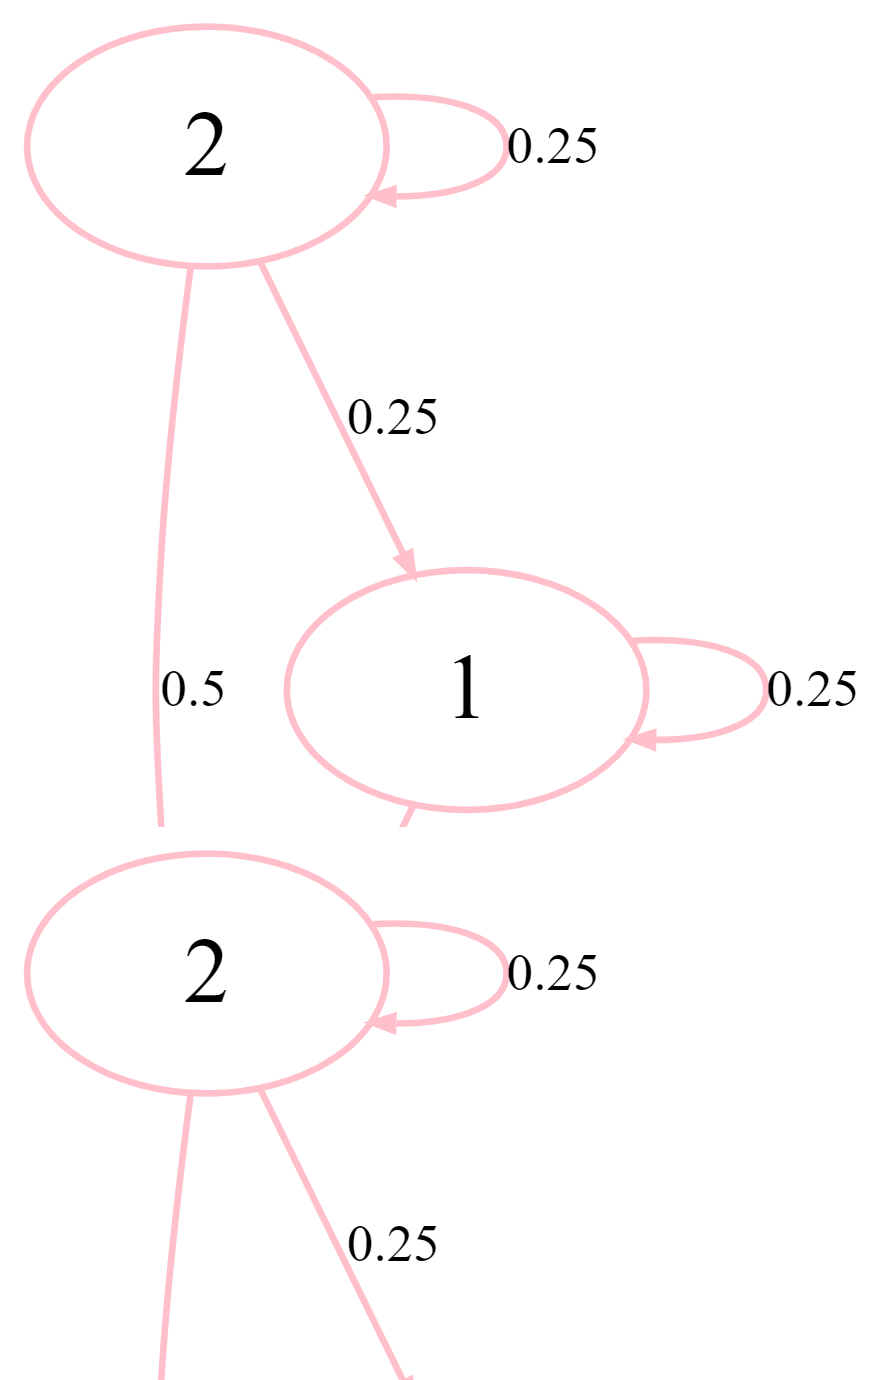
\includegraphics[width=5.5in,height=3.5in]{dinamica_files/figure-latex/dot-figure-1.png}

Para la acción \(a=1\) la cual es admisible cuando el nivel del almacen
es \(0\) o \(1\), tenemos la siguiente tabla de transiciones:

\begin{longtable}[]{@{}
  >{\raggedright\arraybackslash}p{(\columnwidth - 6\tabcolsep) * \real{0.2603}}
  >{\raggedright\arraybackslash}p{(\columnwidth - 6\tabcolsep) * \real{0.2466}}
  >{\raggedright\arraybackslash}p{(\columnwidth - 6\tabcolsep) * \real{0.2466}}
  >{\raggedright\arraybackslash}p{(\columnwidth - 6\tabcolsep) * \real{0.2466}}@{}}
\toprule\noalign{}
\begin{minipage}[b]{\linewidth}\raggedright
x
\end{minipage} & \begin{minipage}[b]{\linewidth}\raggedright
a
\end{minipage} & \begin{minipage}[b]{\linewidth}\raggedright
y
\end{minipage} & \begin{minipage}[b]{\linewidth}\raggedright
\(\mathbf{P}_{x,y}(a)\)
\end{minipage} \\
\midrule\noalign{}
\endhead
\bottomrule\noalign{}
\endlastfoot
contar con \(0\) artículos & solicitar \(1\) artículo & contar con 0
artículos & \(\frac{3}{4}\) \\
contar con \(0\) artículos & solicitar \(1\) artículo & contar con 1
artículos & \(\frac{1}{4}\) \\
contar con \(0\) artículos & solicitar \(1\) artículo & contar con 2
artículos & 0 \\
contar con \(1\) artículo & solicitar \(1\) artículo & contar con 0
artículos & \(\frac{2}{4}\) \\
contar con \(1\) artículo & solicitar \(1\) artículo & contar con 1
artículos & \(\frac{1}{4}\) \\
contar con \(1\) artículo & solicitar \(1\) artículo & contar con 2
artículos & \(\frac{1}{4}\) \\
\end{longtable}

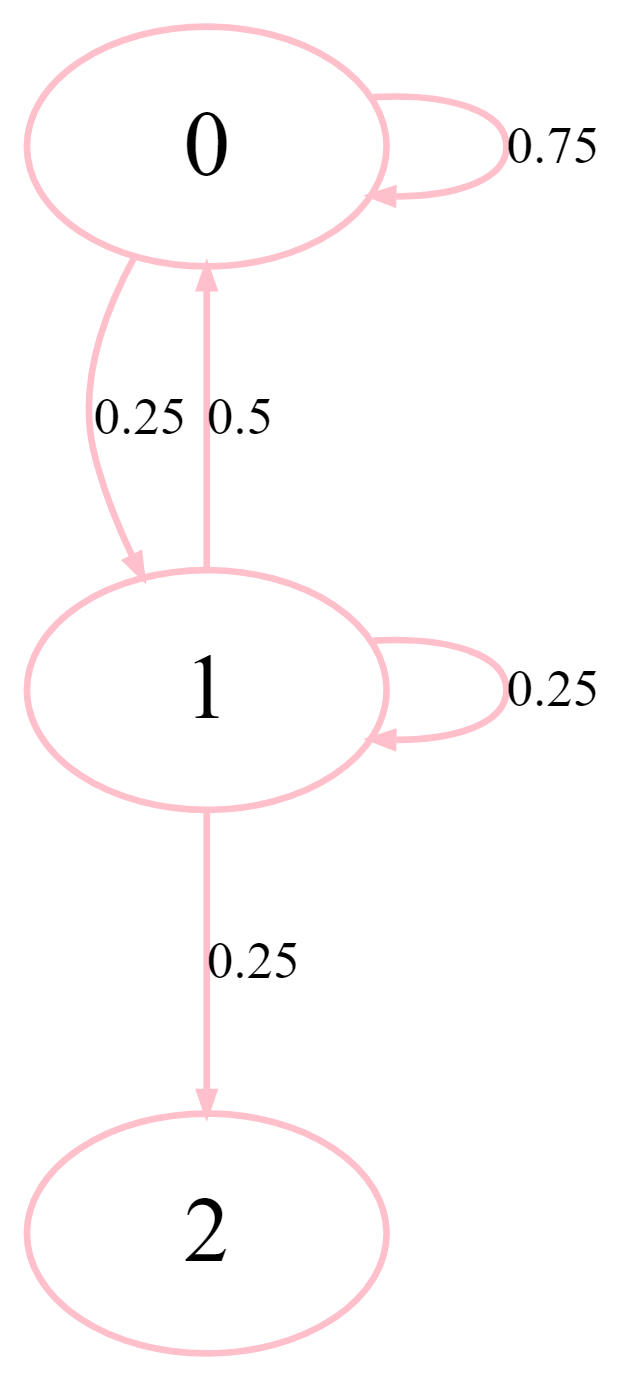
\includegraphics[width=5.5in,height=3.5in]{dinamica_files/figure-latex/dot-figure-3.png}

Para la acción \(a=2\) la cual es admisible únicamente cuando el nivel
del almacen es \(0\) tenemos la siguiente tabla de transiciones:

\begin{longtable}[]{@{}
  >{\raggedright\arraybackslash}p{(\columnwidth - 6\tabcolsep) * \real{0.2653}}
  >{\raggedright\arraybackslash}p{(\columnwidth - 6\tabcolsep) * \real{0.2551}}
  >{\raggedright\arraybackslash}p{(\columnwidth - 6\tabcolsep) * \real{0.2449}}
  >{\raggedright\arraybackslash}p{(\columnwidth - 6\tabcolsep) * \real{0.2347}}@{}}
\toprule\noalign{}
\begin{minipage}[b]{\linewidth}\raggedright
x
\end{minipage} & \begin{minipage}[b]{\linewidth}\raggedright
a
\end{minipage} & \begin{minipage}[b]{\linewidth}\raggedright
y
\end{minipage} & \begin{minipage}[b]{\linewidth}\raggedright
\(\mathbf{P}_{x,y}(a)\)
\end{minipage} \\
\midrule\noalign{}
\endhead
\bottomrule\noalign{}
\endlastfoot
contar con \(0\) artículos & solicitar \(2\) artículos & contar con 0
artículos & \(\frac{2}{4}\) \\
contar con \(0\) artículos & solicitar \(2\) artículos & contar con 1
artículos & \(\frac{1}{4}\) \\
contar con \(0\) artículos & solicitar \(2\) artículos & contar con 2
artículos & \(\frac{1}{4}\) \\
\end{longtable}

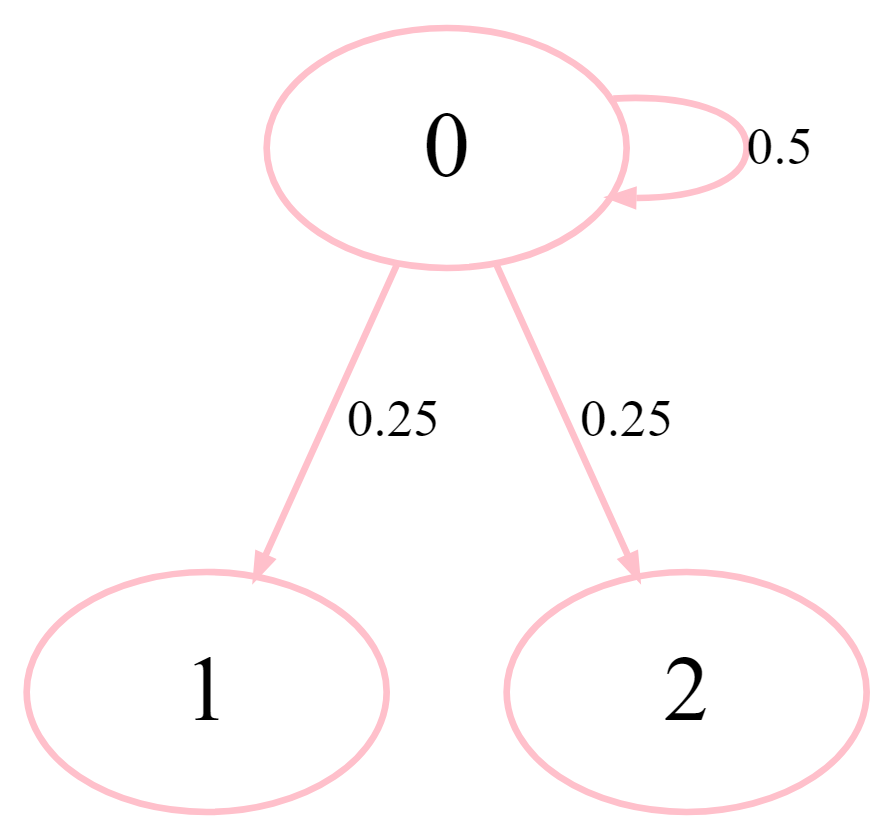
\includegraphics[width=5.5in,height=3.5in]{dinamica_files/figure-latex/dot-figure-2.png}

\bookmarksetup{startatroot}

\chapter{Descripción y Justificación de la Función de
Costo}\label{descripciuxf3n-y-justificaciuxf3n-de-la-funciuxf3n-de-costo}

Para la función de costo por etapa definimos las constantes

\begin{itemize}
\item
  \(\lambda\) : costo unitario de producción.
\item
  \(h\) : costo unitario por almacenamiento
\item
  \(p\): costo unitario por demanda insatisfecha.
\end{itemize}

La función de costo por etapa para cada \((x,a)\) está dada por \[
\mathbf{C}(x,a)=\lambda a+h\max\{0,x_t+a_t-\xi_t\}+p\max\{0,\xi_t-x_t-a_t\}
\] De manera que el costo en cada etapa es igual a la cantidad de
unidades solicitadas a producción, considerando el costo de producción,
mas el costo de almacenamiento, el cual dependerá del producto en
existencia, y considerando que si la demanda excede la producción
almacenada se genera un costo de penalización.

Si el objetivo es mejorar las ganancias a lo largo de \(N\) etapas bajo
el panorama previamente descrito, entonces esto equivale a minimizar el
indice de funcionamiento a continuación \[
J(\pi,x):= \mathbf{E}[\sum_{t=0}^{N-1}\mathbf{C}(x,a)]
\]

\bookmarksetup{startatroot}

\chapter{Justificación de las
Acciones}\label{justificaciuxf3n-de-las-acciones}

Existen modelos en los que se asume que la capacidad del inventario es
infinita, lo cual pocas veces describe la realidad, es por esto que
consideramos que la capacidad con la que contamos es finita, es decir
que las acciones que se pueden realizar al estar a cargo de un
inventario estan limitadas por la capacidad de la bodega y con la
cantidad de producto existente en cada etapa.

\bookmarksetup{startatroot}

\chapter{Simulación del Proceso}\label{simulaciuxf3n-del-proceso}

Para faciltar los calculos se realizó el siguiente codigo en python, con
el cual se genera la sucesión de acciones óptimas y los costos mínimos
en cada etapa de decisión considerando cada estado del sistema

\begin{Shaded}
\begin{Highlighting}[]
\ImportTok{import}\NormalTok{ numpy }\ImportTok{as}\NormalTok{ np}
\ImportTok{import}\NormalTok{ pandas }\ImportTok{as}\NormalTok{ pd}

\CommentTok{\# Parámetros}
\NormalTok{N }\OperatorTok{=} \DecValTok{4} \CommentTok{\# Períodos}
\NormalTok{CosOrd }\OperatorTok{=} \FloatTok{1.2}  \CommentTok{\# Costo por ordenar}
\NormalTok{CosMan }\OperatorTok{=} \DecValTok{3}  \CommentTok{\# Costo por mantener}
\NormalTok{CosEsc }\OperatorTok{=} \DecValTok{4}  \CommentTok{\# Costo por escasez}
\NormalTok{p }\OperatorTok{=}\NormalTok{[}\FloatTok{0.25}\NormalTok{,}\FloatTok{0.25}\NormalTok{,}\FloatTok{0.25}\NormalTok{,}\FloatTok{0.25}\NormalTok{] }\CommentTok{\# Distribución de probabilidad de la demanda}
\NormalTok{MaxCap }\OperatorTok{=} \DecValTok{2}  \CommentTok{\# Máxima capacidad del almacén}
\NormalTok{D }\OperatorTok{=} \DecValTok{3}  \CommentTok{\# Valor máximo de la demanda}

\CommentTok{\# Inicialización de la matriz de costos esperados}
\NormalTok{CostoEsperado }\OperatorTok{=}\NormalTok{ np.zeros((N}\OperatorTok{+}\DecValTok{1}\NormalTok{ , MaxCap }\OperatorTok{+} \DecValTok{1}\NormalTok{))}
\NormalTok{DecisionOptima }\OperatorTok{=}\NormalTok{ np.zeros((N, MaxCap }\OperatorTok{+} \DecValTok{1}\NormalTok{), dtype}\OperatorTok{=}\BuiltInTok{int}\NormalTok{)}

\CommentTok{\# Iteración por etapas}
\ControlFlowTok{for}\NormalTok{ l }\KeywordTok{in} \BuiltInTok{range}\NormalTok{(}\DecValTok{1}\NormalTok{, N }\OperatorTok{+}\DecValTok{1}\NormalTok{):  }\CommentTok{\# Etapas}
    \ControlFlowTok{for}\NormalTok{ s }\KeywordTok{in} \BuiltInTok{range}\NormalTok{(}\DecValTok{0}\NormalTok{, MaxCap }\OperatorTok{+} \DecValTok{1}\NormalTok{):  }\CommentTok{\# Estados}
\NormalTok{        estado }\OperatorTok{=}\NormalTok{ []}
        \ControlFlowTok{for}\NormalTok{ a }\KeywordTok{in} \BuiltInTok{range}\NormalTok{(}\DecValTok{0}\NormalTok{, MaxCap }\OperatorTok{{-}}\NormalTok{ s }\OperatorTok{+} \DecValTok{1}\NormalTok{):  }\CommentTok{\# Acciones}
\NormalTok{            esperado }\OperatorTok{=} \DecValTok{0}
            \ControlFlowTok{for}\NormalTok{ w }\KeywordTok{in} \BuiltInTok{range}\NormalTok{(}\DecValTok{0}\NormalTok{, D }\OperatorTok{+} \DecValTok{1}\NormalTok{):  }\CommentTok{\# Demanda}
\NormalTok{                esperado }\OperatorTok{+=}\NormalTok{ p[w] }\OperatorTok{*}\NormalTok{ (}
\NormalTok{                    CosOrd }\OperatorTok{*}\NormalTok{ a}
                    \OperatorTok{+}\NormalTok{ CosMan }\OperatorTok{*} \BuiltInTok{max}\NormalTok{(}\DecValTok{0}\NormalTok{, s }\OperatorTok{+}\NormalTok{ a }\OperatorTok{{-}}\NormalTok{ w)}
                    \OperatorTok{+}\NormalTok{ CosEsc }\OperatorTok{*} \BuiltInTok{max}\NormalTok{(}\DecValTok{0}\NormalTok{, w }\OperatorTok{{-}}\NormalTok{ s }\OperatorTok{{-}}\NormalTok{ a)}
                    \OperatorTok{+}\NormalTok{ CostoEsperado[l }\OperatorTok{{-}} \DecValTok{1}\NormalTok{, }\BuiltInTok{max}\NormalTok{(}\DecValTok{0}\NormalTok{, s }\OperatorTok{+}\NormalTok{ a }\OperatorTok{{-}}\NormalTok{ w)]}
\NormalTok{                )}
\NormalTok{            estado.append(esperado)}
        \CommentTok{\# Determinación del costo mínimo y la decisión óptima}
\NormalTok{        CostoEsperado[l, s] }\OperatorTok{=}\NormalTok{ estado[}\DecValTok{0}\NormalTok{]}
\NormalTok{        DecisionOptima[l }\OperatorTok{{-}} \DecValTok{1}\NormalTok{, s] }\OperatorTok{=} \DecValTok{0}
        \ControlFlowTok{for}\NormalTok{ a }\KeywordTok{in} \BuiltInTok{range}\NormalTok{(}\DecValTok{1}\NormalTok{, }\BuiltInTok{len}\NormalTok{(estado)):}
            \ControlFlowTok{if}\NormalTok{ estado[a] }\OperatorTok{\textless{}}\NormalTok{ CostoEsperado[l, s]:}
\NormalTok{                CostoEsperado[l, s] }\OperatorTok{=}\NormalTok{ estado[a]}
\NormalTok{                DecisionOptima[l }\OperatorTok{{-}} \DecValTok{1}\NormalTok{, s] }\OperatorTok{=}\NormalTok{ a}

\CommentTok{\# Resultados}
\BuiltInTok{print}\NormalTok{(}\StringTok{"Matriz de Costos Esperados:"}\NormalTok{)}
\BuiltInTok{print}\NormalTok{(CostoEsperado)}
\BuiltInTok{print}\NormalTok{(}\StringTok{"Matriz de Decisiones Óptimas:"}\NormalTok{)}
\BuiltInTok{print}\NormalTok{(DecisionOptima)}
\end{Highlighting}
\end{Shaded}

\begin{verbatim}
Matriz de Costos Esperados:
[[ 0.         0.         0.       ]
 [ 4.95       3.75       3.25     ]
 [ 9.6        8.4        7.475    ]
 [14.25      13.05      12.01875  ]
 [18.9       17.7       16.6421875]]
Matriz de Decisiones Óptimas:
[[1 0 0]
 [1 0 0]
 [1 0 0]
 [1 0 0]]
\end{verbatim}

Los resultados se muetran en las siguientes tablas:

\begin{longtable}[]{@{}llll@{}}
\toprule\noalign{}
\textbf{Épocas de decisión} & \textbf{0} & \textbf{1} & \textbf{2} \\
\midrule\noalign{}
\endhead
\bottomrule\noalign{}
\endlastfoot
3 & 1 & 0 & 0 \\
2 & 1 & 0 & 0 \\
1 & 1 & 0 & 0 \\
0 & 1 & 0 & 0 \\
\end{longtable}

\textbf{Tabla 5.1}: Acción de control óptima

\begin{longtable}[]{@{}llll@{}}
\toprule\noalign{}
\textbf{Épocas de decisión} & \textbf{0} & \textbf{1} & \textbf{2} \\
\midrule\noalign{}
\endhead
\bottomrule\noalign{}
\endlastfoot
3 & 4.95 & 3.75 & 3.25 \\
2 & 9.6 & 8.4 & 7.475 \\
1 & 14.25 & 13.05 & 12.01 \\
0 & 18.9 & 17.7 & 16.642 \\
\end{longtable}

\textbf{Tabla 5.2}: Costos

\bookmarksetup{startatroot}

\chapter*{Referencias}\label{referencias}
\addcontentsline{toc}{chapter}{Referencias}

\markboth{Referencias}{Referencias}

\phantomsection\label{refs}
\begin{CSLReferences}{1}{0}
\bibitem[\citeproctext]{ref-citekey}
Gomez, Jazmín Sarahí Flores. 2022. {«Algoritmo de Aproximación en
Modelos de Control Semi-Markovianos y Markovianos con Costos
Descontados»}. Universidad de Sonora.

\bibitem[\citeproctext]{ref-sargent2024dynamic}
Sargent, Thomas J, y John Stachurski. 2024. {«Dynamic Programming:
Finite States»}. \emph{arXiv preprint arXiv:2401.10473}.

\end{CSLReferences}




\end{document}
